\documentclass[handout, 11pt]{beamer}
\mode
<presentation>{\usetheme{Madrid}}
\institute[UF]{\inst{1}
University of Florida\\
Department of Finance, Insurance, and Real Estate}
\usepackage{adjustbox}
\usepackage{tikz}
\usetikzlibrary{positioning}
\usetikzlibrary{positioning}
\usetikzlibrary{positioning}
\usetikzlibrary{positioning}
\usetikzlibrary{positioning}
\usetikzlibrary{positioning}
\definecolor{darkgreen}{RGB}{31,156,17}
\usepackage{xcolor}
\usepackage{minted}
\usepackage{booktabs}
\setbeamertemplate{headline}{\begin{beamercolorbox}[ht=2.25ex, dp=3.75ex]{section in head/foot}
\insertnavigation{\paperwidth}
\end{beamercolorbox}}
\AtBeginSection{\begin{frame}
\frametitle{Table of Contents}
\tableofcontents[currentsection]
\end{frame}}
\begin{document}
\title[Getting Started]{Getting Started with Python and Excel}
\subtitle{Building a Basic Model in Both Excel and Python}
\author[DeRobertis]{Nick DeRobertis\inst{1}}
\date{\today}
\begin{frame}
\titlepage
\label{title-frame}
\end{frame}
\begin{section}[Basic Problem]{An Introductory Model}
\begin{frame}
\frametitle{Approaching a Problem with Two Tools}
\begin{columns}
\begin{column}{0.5\textwidth}
\vbox to 0.8\textheight{\begin{itemize}
\item The focus today is to get familiar working in both Excel and Python
\vfill
\item We will approach this by building a simple model with both tools
\vfill
\item In later lectures, we will move to combining the tools
\end{itemize}}
\end{column}
\begin{column}{0.5\textwidth}
\vbox to 0.8\textheight{\centering
\vfill
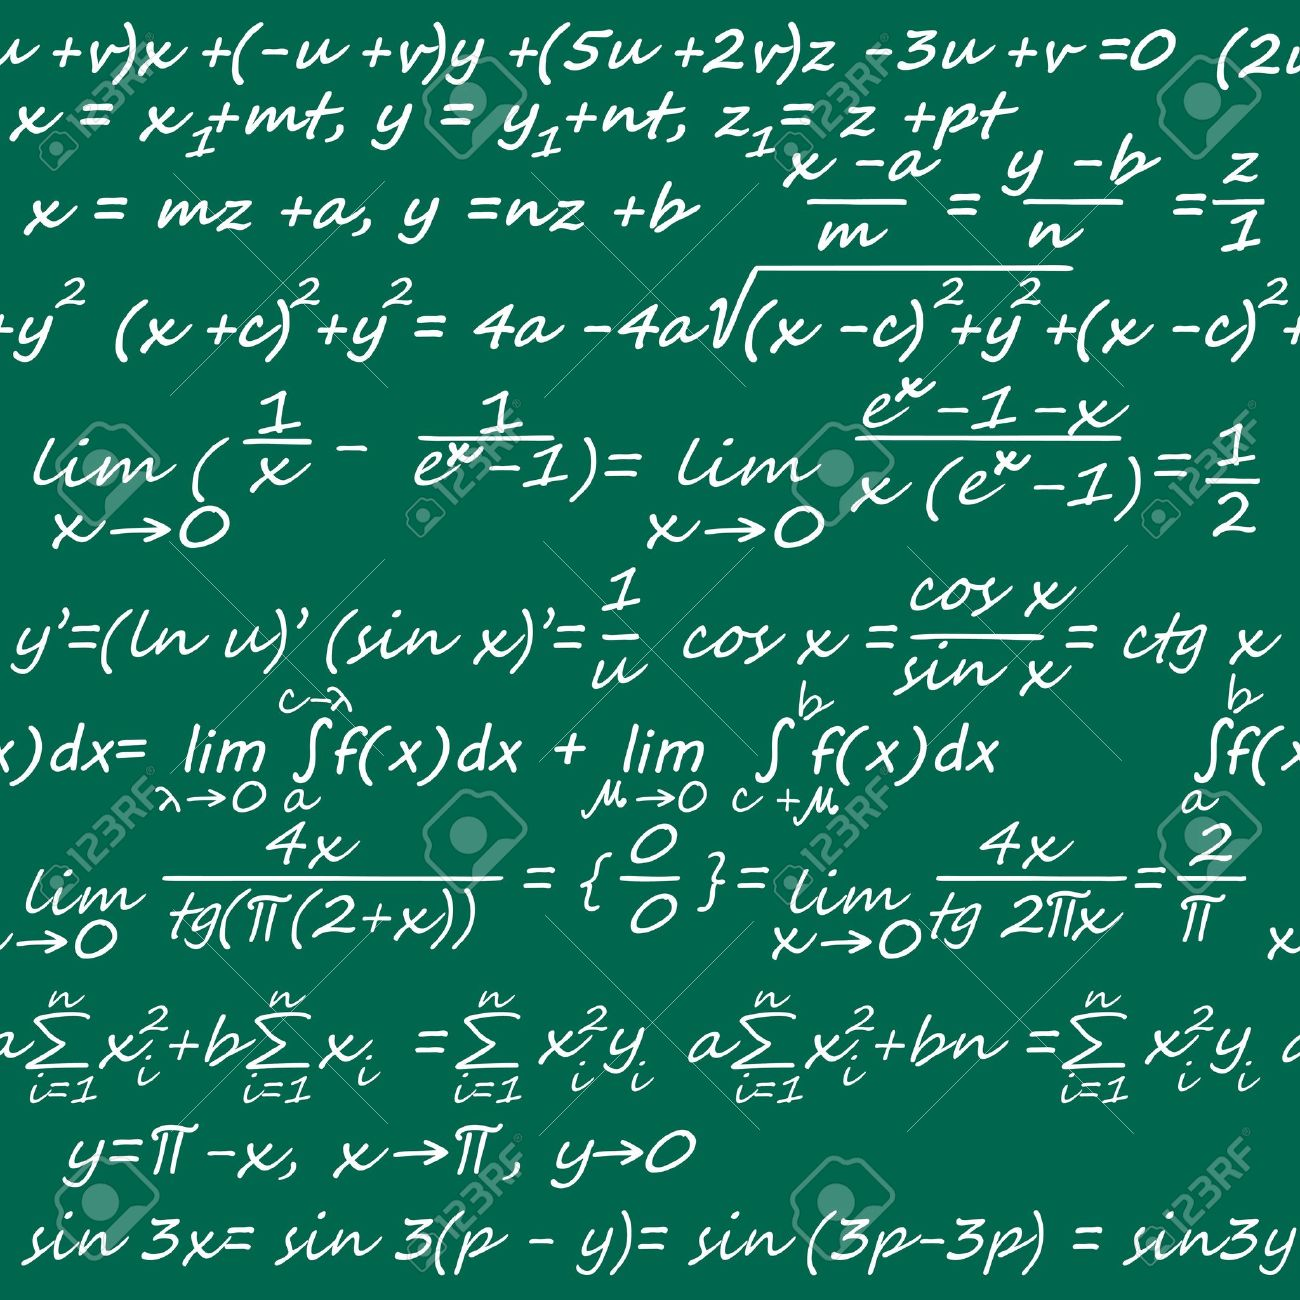
\includegraphics[height=1.0\textheight, keepaspectratio, width=0.9\textwidth]{Sources/equations-chalkboard.jpg}
\vfill
\vfill}
\end{column}
\end{columns}
\end{frame}
\begin{frame}
\frametitle{A Simple Retirement Problem}
\begin{itemize}
\item Let's take what is perhaps the simplest finance problem, which everyone should understand
\vfill
\item While you may have approached such a problem with a calculator before, we will build models for it instead
\vfill
\item Martha is saving for retirement. She earns \$60,000 per year and is able to save 25\% of that. If she invests her savings, earning 5\% per year, and she needs \$1,500,000 to retire, how soon can she retire?
\end{itemize}
\end{frame}
\begin{frame}
\frametitle{Breaking Down the Retirement Problem}
\vspace{-0.25cm}
\begin{block}<+->{A General Structure}
\begin{center}
\begin{adjustbox}{width=0.9\textwidth, height=0.8\textheight, keepaspectratio}
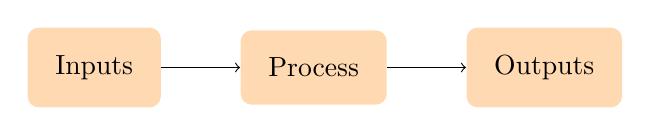
\begin{tikzpicture}
\node [fill=orange!30, rounded corners, inner sep=10pt] (77b7cfc5-f237-4b8b-ade6-b2b41b402949)  {Inputs};
\node [fill=orange!30, rounded corners, inner sep=10pt, right=of 77b7cfc5-f237-4b8b-ade6-b2b41b402949] (170050d0-04a2-4a41-8a84-c7c58c1e31e8)  {Process};
\node [fill=orange!30, rounded corners, inner sep=10pt, right=of 170050d0-04a2-4a41-8a84-c7c58c1e31e8] (4a6151fc-a83a-4b5b-9e7c-e5ffde1e4b60)  {Outputs};
\path [draw, ->] (77b7cfc5-f237-4b8b-ade6-b2b41b402949) -- (170050d0-04a2-4a41-8a84-c7c58c1e31e8);
\path [draw, ->] (170050d0-04a2-4a41-8a84-c7c58c1e31e8) -- (4a6151fc-a83a-4b5b-9e7c-e5ffde1e4b60);
\end{tikzpicture}
\end{adjustbox}
\end{center}
\end{block}
\vspace{-0.25cm}
\begin{block}<+->{Real-world Problem}
\begin{center}
\begin{adjustbox}{width=0.9\textwidth, height=0.8\textheight, keepaspectratio}
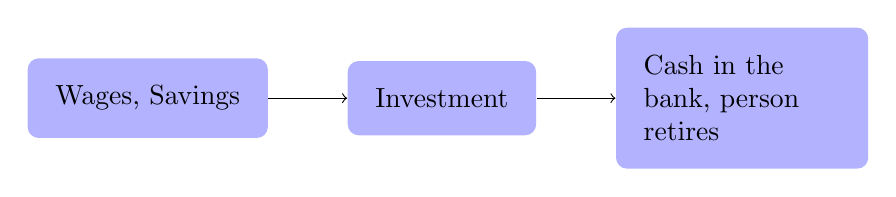
\begin{tikzpicture}
\node [fill=blue!30, rounded corners, inner sep=10pt] (755d7c98-4778-44f2-bbf4-030d2473a6b6)  {Wages, Savings};
\node [fill=blue!30, rounded corners, inner sep=10pt, right=of 755d7c98-4778-44f2-bbf4-030d2473a6b6] (133a4ad1-cb06-49dc-9e20-34fbe122a1bf)  {Investment};
\node [fill=blue!30, rounded corners, inner sep=10pt, text width=2.5cm, right=of 133a4ad1-cb06-49dc-9e20-34fbe122a1bf] (c76dabc2-1964-4a10-b72a-88fafa6f2138)  {Cash in the bank, person retires};
\path [draw, ->] (755d7c98-4778-44f2-bbf4-030d2473a6b6) -- (133a4ad1-cb06-49dc-9e20-34fbe122a1bf);
\path [draw, ->] (133a4ad1-cb06-49dc-9e20-34fbe122a1bf) -- (c76dabc2-1964-4a10-b72a-88fafa6f2138);
\end{tikzpicture}
\end{adjustbox}
\end{center}
\end{block}
\vspace{-0.25cm}
\begin{block}<+->{A Model of the Problem}
\begin{center}
\begin{adjustbox}{width=0.9\textwidth, height=0.8\textheight, keepaspectratio}
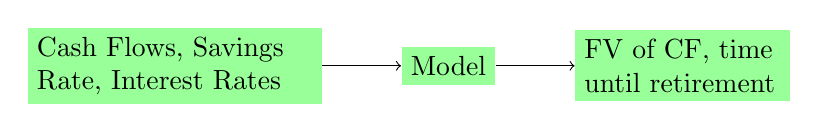
\begin{tikzpicture}
\node [fill=green!40, text width=3.5cm] (ab3d5dad-7dfb-43ae-aa5d-3acc752e0aad)  {Cash Flows, Savings Rate, Interest Rates};
\node [fill=green!40, right=of ab3d5dad-7dfb-43ae-aa5d-3acc752e0aad] (80db54e7-5856-4ac2-83b1-7aaf33e6df66)  {Model};
\node [fill=green!40, text width=2.5cm, right=of 80db54e7-5856-4ac2-83b1-7aaf33e6df66] (f9bf7c24-76fd-46b5-aab1-e33305c3d589)  {FV of CF, time until retirement};
\path [draw, ->] (ab3d5dad-7dfb-43ae-aa5d-3acc752e0aad) -- (80db54e7-5856-4ac2-83b1-7aaf33e6df66);
\path [draw, ->] (80db54e7-5856-4ac2-83b1-7aaf33e6df66) -- (f9bf7c24-76fd-46b5-aab1-e33305c3d589);
\end{tikzpicture}
\end{adjustbox}
\end{center}
\end{block}
\end{frame}
\end{section}
\begin{section}{Excel Solution}
\begin{frame}
\frametitle{Solving the Problem in Excel}
\begin{columns}
\begin{column}{0.5\textwidth}
\vbox to 0.8\textheight{\begin{itemize}
\item It is easy to use Excel as a calculator and just type the math in directly. But we want to build a model.
\vfill
\item Changing inputs should result in a change to outputs. The way to do this in Excel is cell references
\vfill
\item Fixed references become important when trying to drag formulas, e.g. \texttt{\$A\$2} (fully fixed), \texttt{\$A2} (fixed on column), or \texttt{A\$2} (fixed on row).
\end{itemize}}
\end{column}
\begin{column}{0.5\textwidth}
\vbox to 0.8\textheight{\centering
\vfill

\includegraphics[height=1.0\textheight, keepaspectratio, width=0.9\textwidth]{Sources/excel-logo.png}
\vfill
\vfill}
\end{column}
\end{columns}
\end{frame}
\begin{frame}
\frametitle{Simple Retirement Problem in Excel}
{
\setbeamercolor{block title}{bg=darkgreen}
\begin{block}{Intro Excel Exercise}
\begin{itemize}
\item Go to
\textcolor{blue}{\underline{\href{https://nickderobertis.github.io/fin-model-course/}{the course site}}}
and download Simple Retirement Model Excel
\item Follow along as I recreate the simple model.
\end{itemize}
\end{block}
}
\end{frame}
\end{section}
\begin{section}{Python Solution}
\begin{frame}
\frametitle{How We'll Work in Python}
\begin{columns}
\begin{column}{0.5\textwidth}
\vbox to 0.8\textheight{\begin{itemize}
\small
\vfill
\item Using Python in the terminal is kind of a pain. And so, tools were born.
\vfill
\item Jupyter is a graphical interface we can use for Python. It also supports over 40 other languages such as R, SAS, Julia, and Scala
\vfill
\item You can use \texttt{jupyter notebook} or \texttt{jupyter lab}. The latter has a lot more features outside of the notebook. We will focus on using \texttt{jupyter lab} in this class as it is the future of Jupyter.
\end{itemize}}
\end{column}
\begin{column}{0.5\textwidth}
\vbox to 0.8\textheight{\centering
\vfill
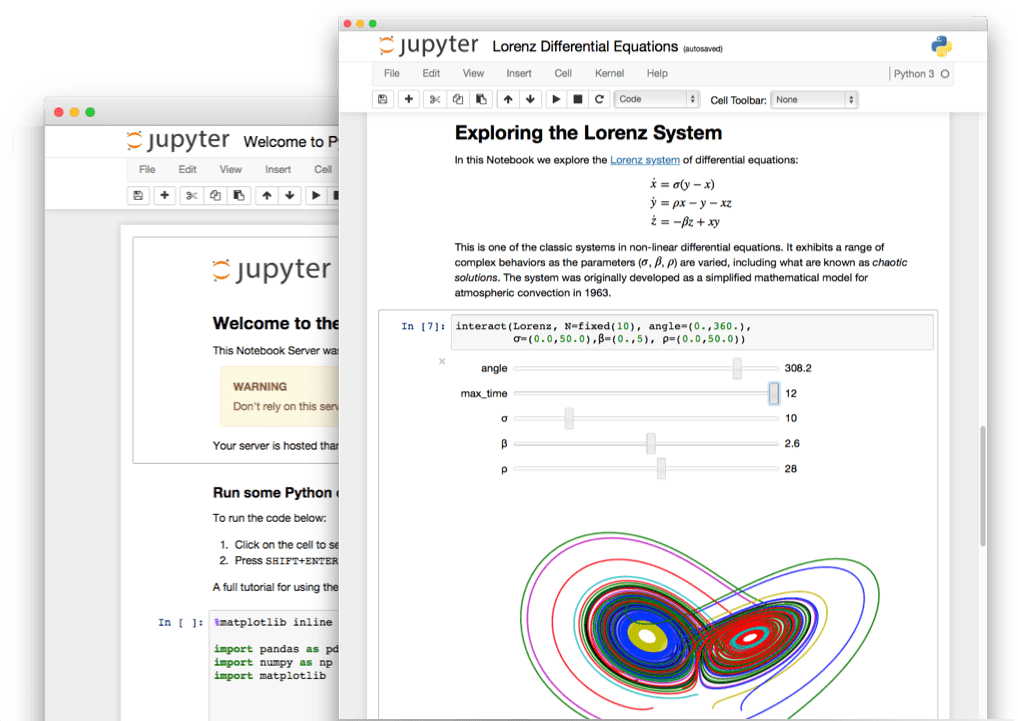
\includegraphics[height=1.0\textheight, keepaspectratio, width=0.9\textwidth]{Sources/jupyter-notebook.png}
\vfill
\vfill}
\end{column}
\end{columns}
\end{frame}
\begin{frame}
\frametitle{Let's Get Set up with Jupyter}
{
\setbeamercolor{block title}{bg=violet}
\begin{block}{Launch Jupyter Notebook}
\begin{enumerate}
\item Launch Anaconda Navigator
\item Find Jupyter Notebook on the main screen, and click launch
\item You should see a list of folders and files. Click New and then Python 3
\item Now you should see a code cell with \texttt{In [ ]:} next to it
\end{enumerate}
\vfill
\end{block}
}
\begin{alertblock}{}
If you don't have Anaconda Navigator, just open a terminal (search \texttt{cmd} on Windows, \texttt{terminal} on Mac). Then in the terminal, type \texttt{jupyter lab} and enter. Then continue with the third step.
\end{alertblock}
\end{frame}
\begin{frame}[fragile]
\frametitle{Some Python Basics}
\begin{itemize}
\item In Excel, the basic unit is a cell. In Python, the basic unit is an object.
\vfill
\item In Excel, content in a cell is either a number (123) or a string (ABC)
\vfill
\item In Python, all objects have types. They might also be a number or a string, or something else.
\vfill
\item Rather than using a cell reference like \texttt{\$A\$2}, we assign names to objects in Python
\vfill
\item \begin{minted}{python}

                        my_number = 6
                        my_string = 'ABC'
                        
\end{minted}
\end{itemize}
\end{frame}
\begin{frame}[fragile]
\frametitle{Doing Some Math in Python}
\begin{columns}
\begin{column}{0.5\textwidth}
\vbox to 0.8\textheight{
\includegraphics[width=1.0\textwidth]{Sources/numpy-logo.png}
\begin{block}{Note: Deprecation warning}
\footnotesize
In the future, these numpy financial functions are being moved to a separate package
\texttt{numpy\_financial}.
For
the purposes of this class, this won't matter, but in the future you may have to install
\texttt{numpy\_financial}
to use these functions.
In the meantime, you will see a warning come up when calling the functions.
\end{block}}
\end{column}
\begin{column}{0.5\textwidth}
\vbox to 0.8\textheight{\begin{itemize}
\item Basic operations in Python are straightforward
\item \begin{minted}{python}
2 + 5 = 7
\end{minted}
\item \begin{minted}{python}
6 - 2 = 4
\end{minted}
\item \begin{minted}{python}
2 * 3 = 6
\end{minted}
\item \begin{minted}{python}
5 / 2 = 2.5
\end{minted}
\item A lot more is available using the \texttt{numpy} package
\item \begin{minted}{python}
np.pv, np.nper,
np.fv, np.pmt
\end{minted}
\item \textcolor{blue}{\underline{\href{https://numpy.org/doc/stable/reference/routines.financial.html}{All numpy financial functions}}}
\end{itemize}}
\end{column}
\end{columns}
\end{frame}
\begin{frame}
\frametitle{Simple Retirement Problem in Python}
{
\setbeamercolor{block title}{bg=darkgreen}
\begin{block}{Intro Python Exercise}
\begin{itemize}
\item Go to
\textcolor{blue}{\underline{\href{https://nickderobertis.github.io/fin-model-course/}{the course site}}}
and download Simple Retirement Model Python
\item In Jupyter, then navigate to your Downloads folder (or wherever you saved it)
\item You should then see Simple Retirement Model.ipynb come up in the list of files in Jupyter. Click it to open it and follow along.
\end{itemize}
\end{block}
}
\end{frame}
\end{section}
\begin{section}[Extend \& Iterate]{Extending the Model and Iteration}
\begin{frame}
\frametitle{Extending the Model - Multiple Interest Rates}
\begin{itemize}
\item Now we've got basic models to determine how long it will take Martha to retire.
\vfill
\item We've got a few assumptions built into the model. One is that Martha will earn 5\% on her investments
\vfill
\item Rates of return are volatile, so we want to see how long it would take her to retire if her return was different
\end{itemize}
\end{frame}
\begin{frame}
\frametitle{Programming Fundamentals - Iteration}
\begin{itemize}
\item In programming, for model building or otherwise, you often need to repeat the same process for multiple different things
\vfill
\item In Excel, you would do this by dragging formulas.
\vfill
\item In Python, as in most other programming languages, we would use a \texttt{for} loop
\vfill
\item This says, do something, for each value I pass into the loop
\end{itemize}
\end{frame}
\begin{frame}[fragile]
\frametitle{Iteration - Python vs. Excel}
\begin{columns}
\begin{column}{0.45\textwidth}
\begin{block}{Python Iteration}
\begin{minted}{python}

inputs = [5, 10, 15]
for item in inputs:
    new_value = item + 2
    print(new_value)

7
12
17
        
\end{minted}
\end{block}
\end{column}
\begin{column}{0.45\textwidth}
\begin{block}{Excel Iteration}
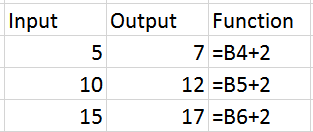
\includegraphics[width=1.0\textwidth]{Sources/excel-iteration.png}
\end{block}
\end{column}
\end{columns}
\end{frame}
\begin{frame}[fragile]
\frametitle{Explaining Python Iteration}
\begin{columns}
\begin{column}{0.5\textwidth}
\vbox to 0.8\textheight{\begin{itemize}
\item There's a few things to unpack here
\item Here's another type of object: not a number or a string, but a \texttt{list}
\item A \texttt{list} holds multiple objects, and you can add or remove items from \texttt{list}s
\end{itemize}}
\end{column}
\begin{column}{0.5\textwidth}
\vbox to 0.8\textheight{\begin{block}{Python Iteration}
\begin{minted}{python}

inputs = [5, 10, 15]
for item in inputs:
    new_value = item + 2
    print(new_value)

7
12
17
        
\end{minted}
\end{block}}
\end{column}
\end{columns}
\end{frame}
\begin{frame}[fragile]
\frametitle{Explaining Python Iteration (pt. 2)}
\begin{columns}
\begin{column}{0.5\textwidth}
\vbox to 0.8\textheight{\begin{itemize}
\item Here we define a list of three numbers as inputs
\item Then we use a \texttt{for} loop to get each input out of the list, and add 2 to it to create the new value
\item Finally we print each value as it is generated
\end{itemize}}
\end{column}
\begin{column}{0.5\textwidth}
\vbox to 0.8\textheight{\begin{block}{Python Iteration}
\begin{minted}{python}

inputs = [5, 10, 15]
for item in inputs:
    new_value = item + 2
    print(new_value)

7
12
17
        
\end{minted}
\end{block}}
\end{column}
\end{columns}
\end{frame}
\begin{frame}
\frametitle{Iterating the Existing Model}
{
\setbeamercolor{block title}{bg=darkgreen}
\begin{block}{Expanding on Python and Excel}
\begin{itemize}
\item I will now expand the existing Excel and Python models to examine multiple interest rates
\item Continue viewing the same previously downloaded files.
\end{itemize}
\end{block}
}
\end{frame}
\begin{frame}
\frametitle{Vary Savings Rate Lab}
{
\setbeamercolor{block title}{bg=violet}
\begin{block}{Extending a Simple Retirement Model}
\begin{enumerate}
\item Now we want to see the effect of savings rate on time until retirement, in addition to interest rate
\item In both Excel and Python, calculate the years to retirement for savings rates of 10\%, 25\%, and 40\%, and each of these cases with each of the interest rate cases, 4\%, 5\%, and 6\%
\item Be sure that you drag formulas in Excel and use for loops in Python to accomplish this
\item In total you should have 9 calculated years to retirement numbers, in each of the two models.
\end{enumerate}
\vfill
\begin{tabular*}{\textwidth}{@{\extracolsep{\fill}}cccc}
\toprule
\hfill & Answers: Slide \textcolor{blue}{\underline{\ref{labs:vary-savings-rate-lab-1-answers}}} & Resources: Slide \textcolor{blue}{\underline{\ref{labs:vary-savings-rate-lab-1-resources}}} & \hfill\\

\end{tabular*}
\end{block}
}
\label{labs:vary-savings-rate-lab-1}
\end{frame}
\end{section}
\appendix
\newcounter{finalframe}
\setcounter{finalframe}{\value{framenumber}}
\begin{frame}
\frametitle{Lecture Resources}
{
\setbeamercolor{block title}{bg=teal}
\begin{block}{Lecture Resources}
\begin{enumerate}
\item \textcolor{blue}{\underline{\href{https://nickderobertis.github.io/fin-model-course/\_static/generated/pdfs/S2 Getting Started with Python and Excel.pdf}{Slides - Getting Started with Python and Excel}}}
\item \textcolor{blue}{\underline{\href{https://nickderobertis.github.io/fin-model-course/\_static/generated/pdfs/LN2 Getting Started with Python and Excel.pdf}{Lecture Notes - Getting Started with Python and Excel}}}
\item \textcolor{blue}{\underline{\href{https://nickderobertis.github.io/fin-model-course/\_static/Examples/Introduction/Excel/Simple Retirement Model.xlsx}{Simple Retirement Model - Excel}}}
\item \textcolor{blue}{\underline{\href{https://nickderobertis.github.io/fin-model-course/\_static/Examples/Introduction/Python/Simple Retirement Model.ipynb}{Simple Retirement Model - Python}}}
\end{enumerate}
\vfill
\end{block}
}
\label{frames:resources}
\end{frame}
\small
\begin{frame}
\frametitle{Vary Savings Rate Lab, Answers}
{
\setbeamercolor{block title}{bg=orange}
\begin{block}{Extending a Simple Retirement Model, Answers}
\begin{enumerate}
\item Martha has 61.1 years to retirement if she earns a 4\% return and saves 10\%.
\item Martha has 41.0 years to retirement if she earns a 4\% return and saves 25\%.
\item Martha has 31.9 years to retirement if she earns a 4\% return and saves 40\%.
\item Martha has 53.3 years to retirement if she earns a 5\% return and saves 10\%.
\item Martha has 36.7 years to retirement if she earns a 5\% return and saves 25\%.
\item Martha has 29.0 years to retirement if she earns a 5\% return and saves 40\%.
\item Martha has 47.6 years to retirement if she earns a 6\% return and saves 10\%.
\item Martha has 33.4 years to retirement if she earns a 6\% return and saves 25\%.
\item Martha has 26.7 years to retirement if she earns a 6\% return and saves 40\%.
\end{enumerate}
\vfill
\begin{tabular*}{\textwidth}{@{\extracolsep{\fill}}cccc}
\toprule
\hfill & Exercise: Slide \textcolor{blue}{\underline{\ref{labs:vary-savings-rate-lab-1}}} & Resources: Slide \textcolor{blue}{\underline{\ref{labs:vary-savings-rate-lab-1-resources}}} & \hfill\\

\end{tabular*}
\end{block}
}
\label{labs:vary-savings-rate-lab-1-answers}
\end{frame}
\begin{frame}
\frametitle{Vary Savings Rate Lab Resources}
{
\setbeamercolor{block title}{bg=teal}
\begin{block}{Extending a Simple Retirement Model Resources}
\begin{enumerate}
\item \textcolor{blue}{\underline{\href{https://nickderobertis.github.io/fin-model-course/\_static/Examples/Introduction/Excel/Simple Retirement Model.xlsx}{Simple Retirement Model - Excel}}}
\item \textcolor{blue}{\underline{\href{https://nickderobertis.github.io/fin-model-course/\_static/Examples/Introduction/Python/Simple Retirement Model.ipynb}{Simple Retirement Model - Python}}}
\item \textcolor{blue}{\underline{\href{https://nickderobertis.github.io/fin-model-course/\_static/generated/pdfs/S2 Getting Started with Python and Excel.pdf}{Slides - Getting Started with Python and Excel}}}
\end{enumerate}
\vfill
\begin{tabular*}{\textwidth}{@{\extracolsep{\fill}}cccc}
\toprule
\hfill & Exercise: Slide \textcolor{blue}{\underline{\ref{labs:vary-savings-rate-lab-1}}} & Answers: Slide \textcolor{blue}{\underline{\ref{labs:vary-savings-rate-lab-1-answers}}} & \hfill\\

\end{tabular*}
\end{block}
}
\label{labs:vary-savings-rate-lab-1-resources}
\end{frame}
\normalsize
\setcounter{framenumber}{\value{finalframe}}
\end{document}